

	
	
 	\begin{figure} 
 		\centering
 		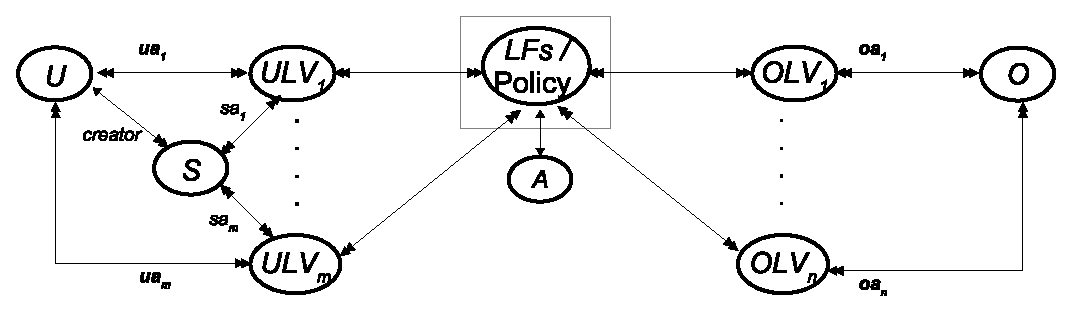
\includegraphics[width=.9\textwidth]{DBSEC16/lpabac-mn}
 		\caption{Components of \LPModels{} model with m user and n object attributes}
 		\label{fig:lp-abacmn-diagram}
 	\end{figure}
	
	
	\label{sec:models}
	%In this section, we define a multi-attribute enumerated authorization policy ABAC model named \EPMNModel{} (shown in Figure \ref{fig:epabac-mn}). To the best of our knowledge, \EPMNModel{} is the first such model. \PM{}\cite{policy-machine} also defines a multi-attribute \EPModels{} model, but their interpretation of attributes is different than the traditional interpretation of \textit{(attribute-name, value)} pairs. 
	
	We also define a multi-attribute \LPModels{} model named \LPMN{} (shown in Figure \ref{fig:lp-abacmn-diagram})  by abstracting its policy language and potentially accepting any computational logic as policy language. While existing \LPModels{} models  define their own policy language, \LPMN{} can subsume any policy language which further generalizes our equivalence results presented in the following section.  The differences between \EPMNModel{} and \LPMN{} are highlighted in boxes in the figures. 
	


		%\vspace{-1em}
\begin{table}[t]
	\centering
	\caption{ \LPMN{} model} %\vspace*{3pt}
	\label{tab:lp-abacmn-definition}
		\begin{tabular}{|l|}						
		\hline					
				\multicolumn{1}{|c|}{\underline{\textit{I. Sets and relations}}}\\			
				 - $U, O$, $S, A$ (set of users,  objects , subjects and actions resp.)\\
				 %- $ \UAV, \textit{\OAV}$ and $A$ (finite set of user and object attribute values and actions resp.) \\
				 - $\UAV{1}, \UAV{2}, ..., \UAV{m}$ (range of user attribute functions) \\
				 - $\OAV{1}, \OAV{2}, ..., \OAV{n}$ (range of object attribute functions) \\
				 - $UA = \{\ua{1}, \ua{2}, ..., \ua{m}\}$ (set of all user attributes);   $\ua{i}: U \to 2^{\UAV{i}}$ for $1 \le i \le m$\\
 				 -  $OA = \{\oa{1}, \oa{2}, ..., \oa{n}\}$ (set of all object attributes); $\oa{i}: O \to 2^{\OAV{i}}$ for $1 \le i \le n$\\
  			     - $\creator: S \to U$, many-to-one mapping \\
 				 - $SA = \{\sa{1}, \sa{2}, ..., \sa{m}\}$ (set of all subject attributes); $\sa{i}(s) \subseteq \ua{i}(\creator(s))$\\	
				
				%$\langle$ see Table \ref{tab:abac11-session} for user level session functions $\rangle$ \\
				
				 \multicolumn{1}{|c|}{\underline{\textit{II. Policy components}}} \\						
				
				-  $f_a: (2^{\UAV{1}}, 2^{\UAV{2}}, ... ,2^{\UAV{m}}, 2^{\OAV{1}},  2^{\OAV{2}}, ... , 2^{\OAV{n}} )\to \{true, false\}$ (policy for $a \in A$).  \\
   			    - $LFs = \{f_a | a \in A \} $ ( set of all policies)\\			
				 
				
				 \multicolumn{1}{|c|}{\underline{\textit{III. Authorization function}}} \\						
				- \request(s:S,\amem:A,\objmem:O) = \\	\hfill  $\exists f_a \in LFs[f_a(\sa{1}(s), \sa{2}(s),..., \sa{m}(s),  \oa{1}(o), \oa{2}(o), ... \oa{n}(o)) = true] $  
			
\\ \hline	
	\end{tabular}
	
\end{table}

%\vspace{-1em}


	
	
	
	


\subsubsection{\LPMN{} - a multi-attribute logical-formula authorization policy ABAC model.}
	\label{sec:lpmodels}
	 
	  
 	\begin{figure} 
 		\centering
 		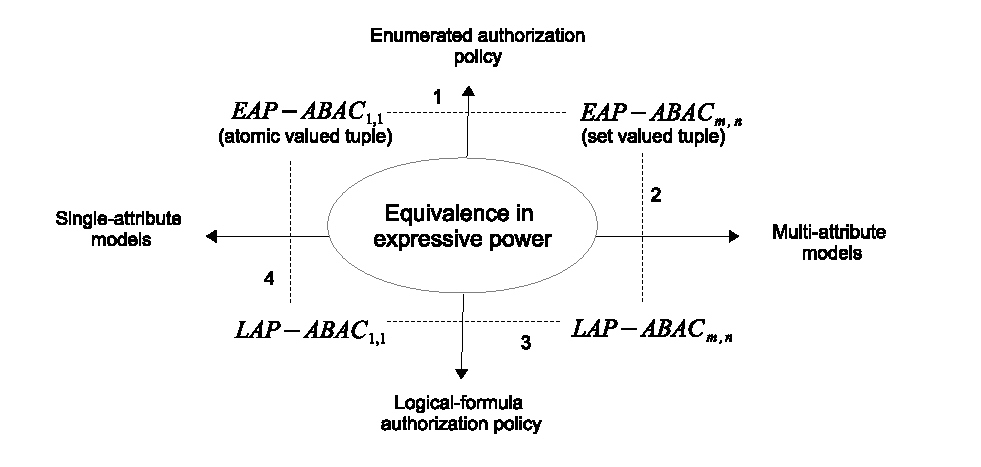
\includegraphics[width=.9\textwidth]{DBSEC16/all-equivalence}
 		\caption{Equilavence of enumerated and logical-formula auth. policy ABAC models}
 		\label{fig:all-equivalence}
 	\end{figure}
 

	 \LPMN{} (given in Figure \ref{fig:lp-abacmn-diagram}) is very similar to \EPMNModel{}, except it is based on LAPs.  It has an unbounded set of users, objects and sessions and a finite set of user attributes, object attributes, session attributes and authorization policies. \LPMN{} does not define an concrete policy language. Instead, it defines  authorization policies as any boolean function that takes values of $m$ subject and $n$ object attributes as parameters. If attribute values of a requesting subject, and requested object evaluate the authorization function $f_a$ (defined for action $a \in A$) true, corresponding access is granted. The formal definition of the model is given in Table \ref{tab:lp-abacmn-definition}. We deliberately maintain similar sets and relations (compare to \EPMNModel{})  to assert that these models only differ in the definition of authorization policies. 
	 

	
